\documentclass[class=report, crop=false, 12pt,a4paper, tikz, border=4mm]{standalone}
\usepackage{enumitem}
\usepackage{float}
\usepackage{amsmath}
\usepackage{amssymb}
\usepackage[normalem]{ulem}
\usepackage{graphicx}
\usepackage{siunitx}
\usepackage{tikz}
\usetikzlibrary{positioning, fit, calc}   
\tikzset{block/.style={draw, thick, text width=3cm ,minimum height=1.3cm, align=center},   
line/.style={-latex}     
}
\begin{document}
\section{Strain gauges}
\subsection{Strain}
The changes in the value of a dimension of a body divided by the original value of the dimension is the relative change in the dimensions. 
\begin{figure}[H]
  \centering
  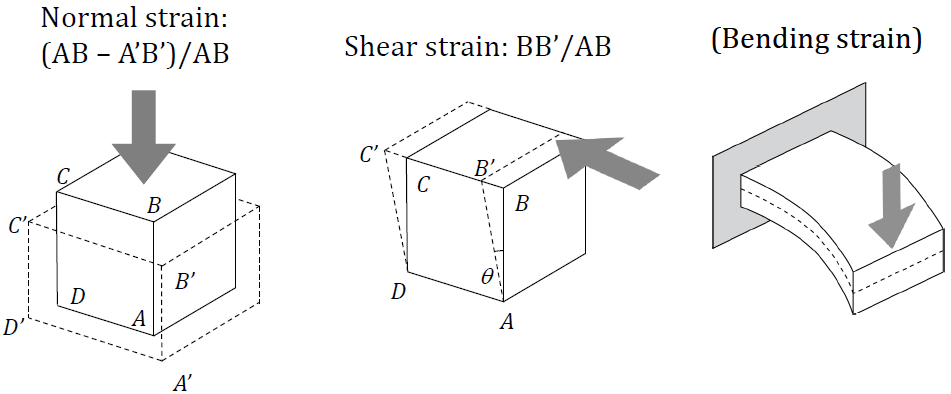
\includegraphics[width = 0.8 \textwidth]{../img/diagram8.png}
\end{figure}
Information about strain is required in many engineering situations: an aircraft in flight, support pillars and spans of bridges, etc.
\subsection{Stress}
Density of the reactive (internal) forces distributed throughout the body (force per unit area), in response to external force. Types of stress:
\begin{itemize}
  \item Tensile/compressive stress
  \item Shear stress
  \item Bending stress
\end{itemize}
Elastic modulus:
\begin{equation}
  E = \frac{\textrm{stress}}{\textrm{strain}}
\end{equation}
\begin{itemize}
  \item Young's modulus - normal strain (and if relationship is linear)
  \item Shear modulus - shear strain
  \item Bulk modulus - volumetric strain
\end{itemize}
\subsection{Strain gauges}
A device which experiences a change of electric resistance when it is strained. A strain gauge is combined with other electrical components to obtain an electric voltage or current representing tensile, compressive or bending strain, together wit the means of displaying or recording its value. The total resistance of a block of conducting material of uniform cross section $A$ and length $l$:
\begin{equation}
  R = \rho \frac{l}{A}
  \label{resistance}
\end{equation}
Where $\rho$ is resistivity with units \si{\ohm \meter}.
\begin{figure}[H]
  \centering
  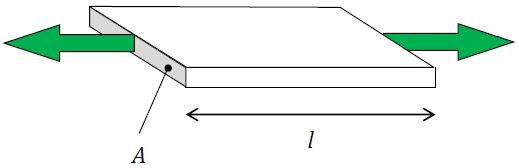
\includegraphics[width = 0.8 \textwidth]{../img/diagram9.png}
  \caption{When the block is subjected to a tensile stress, its length will increase and cross-sectional area will decrease, both of which cause the resistance to increase according to equation (\ref{resistance})}
\end{figure}
The resistivity of the material will also change because of the \textbf{piezo-resistive effect} (increase with tension and decrease with compression). The resistance of the block can thus be written as:
\begin{equation}
  R' = (\rho + \delta \rho) \frac{l + \delta l}{A - \delta A}
\end{equation}
Note: compressive stress will result in a decrease in total resistance.
\subsection{Simple wire strain gauge}
A long fine wire is folded to fit in a small area and then mounted on a flexible backing sheet, usually paper. When \textbf{firmly stuck} to the surface of a much more rigid body, any deformation of this body will cause an identical fractional change of the strain gauge wire. The change of resistance for any strain along the active axis will be much greater than for an equal strain occurring along the passive axis.
\begin{figure}[H]
  \centering
  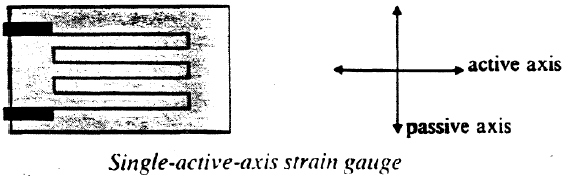
\includegraphics[width = 0.8 \textwidth]{../img/diagram10.png}
\end{figure}
\subsection{Gauge factor}
Defined as the fractional change of resistance of the gauge, divided by the fractional change in the length of the gauge along the active axis:
\begin{equation}
  G = \frac{\frac{\Delta R}{R}}{\frac{\Delta l}{l}}
\end{equation}
Since $\frac{\Delta l}{l}$ is the strain $e$ in the body to which the gauge is fixed, this can be rewritten as:
\begin{equation}
  \frac{\Delta R}{R} = eG
\end{equation}
Most gauges have a $G$ between \textbf{1.8 to 2.2}, depending on the gauge material and the magnitude of the piezo-resistive effect.
\subsection{Foil strain gauge}
Most modern strain gauges are formed by rolling out a thin foil of the resistive material and then cutting away parts of the foil by a photo-etching process, to create the required grid pattern.
\begin{itemize}
  \item Usually supplied with think backing paper as electrical insulation
  \item Adhesive layer for the fixation to the specimen should be creep-free and allow heat dissipation
\end{itemize}
Advantages over simple wire strain gauges:
\begin{itemize}
  \item Larger surface area results in a larger area of adhesion
  \item Accurate reproducibility due to photo-etching technique
  \item Small dimensions mean they are good for localised strain, fit well to curvature
\end{itemize}
\subsection{How can we measure strain}
\begin{figure}[H]
  \centering
  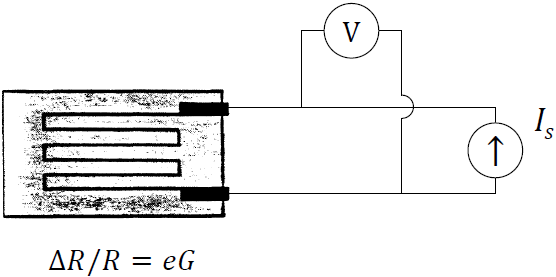
\includegraphics[width = 0.8 \textwidth]{../img/diagram11.png}
  \caption{Is this good enough?}
\end{figure}
Typically $e = 10^{-3}, \ G = 2.1, \ R = 120 \si{\ohm}, \ I_S < 50 \si{\milli \ampere}$.
\begin{gather}
  V = 6 \si{\volt}, \ \Delta R = 0.252 \si{\ohm}\\
  \Delta V = 0.013 \si{\volt}
\end{gather}
The fractional change of the voltage is too small to detect comparing to the 'baseline' voltage $(=RI_S)$.
\section{Wheatstone bridge}
Used to convert the change of resistance in the strain gauge into an electrical signal which could be used to indicate the value of strain. With this, \textbf{zero strain $\leftrightarrow$ zero output voltage}.
\begin{figure}[H]
  \centering
  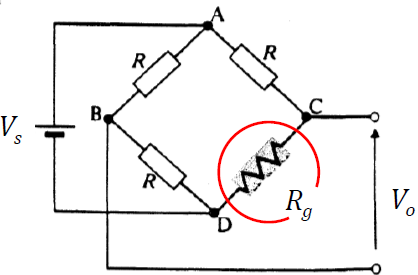
\includegraphics[width = 0.6 \textwidth]{../img/diagram12.png}
\end{figure}
Here, 
\begin{equation}
  V_C - V_D = \frac{V_S R_G}{R + R_G}
\end{equation}
and then,
\begin{equation}
  V_0 = V_C - V_B = \left( V_D + \frac{V_S R_G}{R + R_G} \right) - \left( V_D + \frac{V_S}{2} \right) = \frac{V_S R_G}{R + R_G} - \frac{V_S}{2}
\end{equation}
$R$ is chosen to have the same value as the unstrained gauge, i.e. $R = R_G$ when zero strain $\rightarrow V_0 = 0$ when zero strain. When the gauge is strained, $R_G = R + r$ and the output voltage is
\begin{equation}
  V_0 = V_S \frac{R + r}{2R + r} - \frac{V_S}{2} = V_S \frac{r}{2(2R +r)}
\end{equation}
Now using the gauge factor, $\frac{r}{R} = eG$ and the equation can be rewritten: 
\begin{equation}
  V_0 = V_S \frac{ReG}{2(2R + ReG)} = V_S\frac{eG}{2(2+eG)} \approx \frac{1}{4} V_S eG
\end{equation}
Because typically $eG < 0.02 << 2$

Sensitivity:
\begin{equation}
  \frac{V_0}{e} = \frac{1}{4} V_S G
\end{equation}
\subsection{Temperature compensation}
The output voltage from the strain gauge and the bridge also depends on the temperature. Changes in temperature will cause changes in:
\begin{itemize}
  \item Dimensions of the specimen and hence the gauge due to thermal expansion
  \item Dimensions of the gauge itself (particularly thickness)
  \item Resistivity of the gauge material
\end{itemize}
Compensated with a dummy gauge:
\begin{figure}[H]
  \centering
  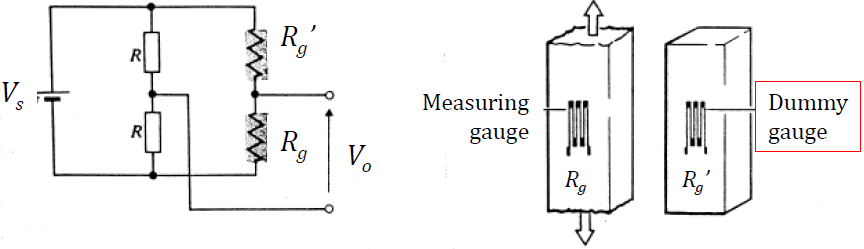
\includegraphics[width = 0.8 \textwidth]{../img/diagram13.png}
\end{figure}
The output voltage of the bridge is: 
\begin{equation}
  V_0 = V_S \frac{R_G}{R_G + R_G'} - \frac{V_S}{2}
\end{equation}
Substituting for $R_G$ and $R_G'$, we have:
\begin{gather}
  V_0 = V_S \frac{R(1+x){1+y}}{R(1+x){1+y} + R(1+y)} - \frac{V_S}{2}\\
  \frac{V_0}{V_S} = \frac{R(1+x){1+y}}{R(1+x){1+y} + R(1+y)} - \frac{1}{2} \leftarrow \textrm{no influence by y}
\end{gather}
However, for this you must find the specimen of the same material and keep them under the same temperature - are these easy enough? The dummy gauge could be placed on the same member as the measuring gauge with its active axis in the direction normal to that of the strain.
\subsection{Effect of Poisson's ratio on a dummy gauge}
Consider both measuring and dummy gauges are attached to the same specimen but perpendicular to each other.
\begin{figure}[H]
  \centering
  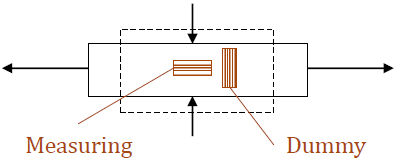
\includegraphics[width = 0.6 \textwidth]{../img/diagram14.png}
\end{figure}
Deformation of the specimen elongates the measuring gauge and shortens the dummy gauge, and the ratio of strains in the two directions is Poisson's ratio, $v = e_{\textrm{lateral}}/e_{\textrm{longitudinal}}$, which is between 0.25 to 4 for most materials. Ignoring temperature changes, the measuring gauge and dummy gauge resistances are then \begin{align}
  R_g &= R(1+x)\\
  R_g' &= R(1-\nu x)
\end{align}
The bridge output is: 
\begin{equation}
  V_0 = V_S\frac{R_g}{R_g + R_g'} - \frac{V_S}{2}
\end{equation}
Substituting for $R_g$ and $R_g'$, we have:
\begin{align}
  V_0 &= V_S \frac{R(1+x)}{R(1+x) + R_g(1-\nu x)} - \frac{V_S}{2}\\
  \frac{V_0}{V_S} &= \frac{R(1+x)}{R(1+x) + R_g(1-\nu x)} - \frac{1}{2}\\
  \frac{V_0}{V_S} &= \frac{(1+ \nu)}{2[2+ (1-\nu)x]} \approx \frac{1}{4} (1+\nu) eG
\end{align}
Because typically $(1-\nu) x << 2$. Comparing to the single gauge, $\frac{V_0}{V_S} = \frac{1}{4}eG$, sensitivity is increased by a factor $(1+\nu)$ due to the effect of Poisson's ratio on the dummy gauge.
\section{Practical Aspects of Strain Gauge Measurement}
\subsection{Strain gauge rosette}
\begin{figure}[H]
  \centering
  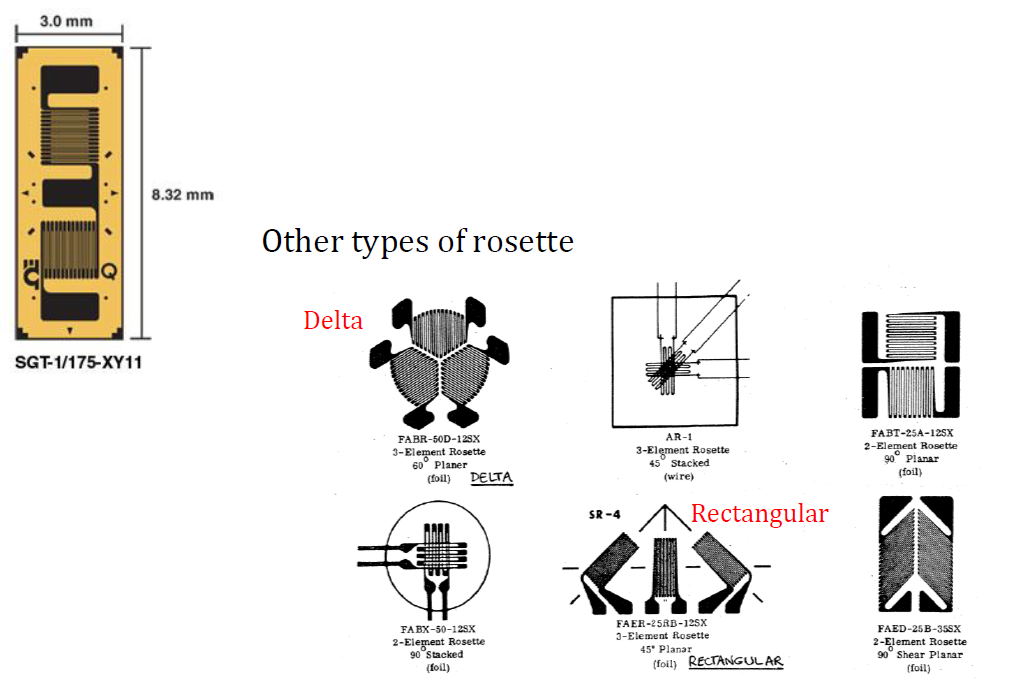
\includegraphics[width = 0.8 \textwidth]{../img/diagram15.png}
  \caption{An example of a foil strain gauge having two elements with their active axis perpendicular to each other is shown in the top left (Omega Engineering Inc. USA). Some other types of rosette are also shown (figures courtesy of BLH Electronics, Waltham, Mass )}
\end{figure}
How can be these useful? Strain (stress) in real-world applications is, not uniformly distributed and/or the principal stress axis is unknown. We use strain gauge rosettes to measure strain in three orientations. Understand complex stress/strain state (principal stress calculation is a topic of MECH0013 in term 2).
\subsection{Bending Strain}
To measure the strain of a member in which only bending is occurring, i.e. no additional tensile or compressive stresses present, we attach two strain gauges one on either side of its neutral axis with their actives axes along the length of the member.
\begin{figure}[H]
  \centering
  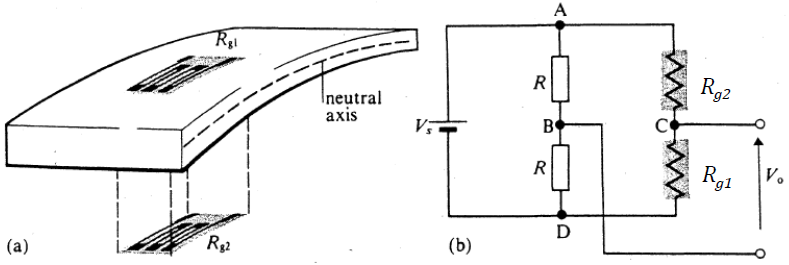
\includegraphics[width = 0.8 \textwidth]{../img/diagram16.png}
\end{figure}
If the gauges are equidistant from the neutral axis, the tensile strain imposed on one will be equal to the compressive strain in the other, and t he change of the resistance is the same magnitude but in opposite directions. Similarly to the previous cases, consider the fractional change of resistance $x$ and then output voltage.
\begin{align}
  V_0 &= V_S \frac{R_{g1}}{R_{g1} + R_{g2}} - \frac{V_S}{2}\\
  &= V_S \frac{R(1+x)}{R(1+x) + R(1-x)} - \frac{V_S}{2} = \frac{1}{2} V_S x
\end{align}
Since $x=eG, \ V_0 = \frac{1}{2} V_S eG$ is a measure of bending occurring in the body.
\subsection{Tensile or compressive strain in a bending member}
The arrangement shown below allows to measure any tensile or compressive strain in the member, while ignoring any bending strain.
\begin{figure}[H]
  \centering
  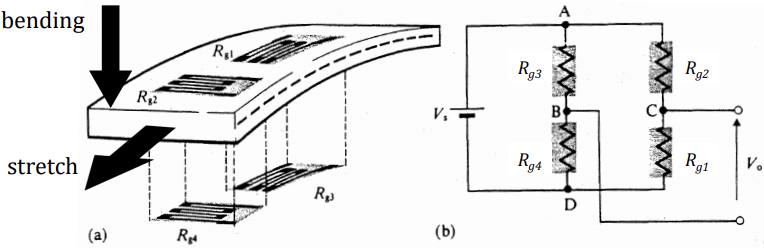
\includegraphics[width = 0.8 \textwidth]{../img/diagram17.png}
  \caption{Variation of gauge resistance and output voltage in the configuration above.}
\end{figure} 
\begin{center}
  \begin{tabular}{||c | c c c c c||} 
    \hline
    & $Rg_1$ & $Rg_2$ & $Rg_3$ & $Rg_4$ & $V_0$\\
    \hline
    Under pure stretch & ++ & - & ++ & - & ++\\
    Under pure bending & ++ & - & - - & + & $\pm 0$ \\
    \hline 
 \end{tabular}
\end{center}
\subsection{Bridge balancing}
In reality, resistance in the arms of the Wheatstone bridge slightly differ in value because of: 
\begin{itemize}
  \item Manufacturing variations
  \item Temperature differences between gauges and resistors
  \item Static strain occurring in a member
\end{itemize}
\begin{figure}[H]
  \centering
  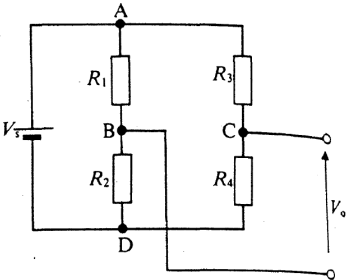
\includegraphics[width = 0.6\textwidth]{../img/diagram18.png}
\end{figure}
If the bridge is perfectly balanced:
\begin{gather}
  \frac{R_4}{R_3 + R_4} = \frac{R_2}{R_1 +R_2}\\
  \rightarrow \frac{R_3}{R_4} + 1 = \frac{R_1}{R_2} +1 \rightarrow \frac{R_3}{R_4} = \frac{R_1}{R_2}
\end{gather}
The imbalance needs to be adjusted before the measurement (adjustment of the output voltage to zero) $\rightarrow$ bridge balancing. One possible way to achieve this is to connect a pot (potentiometer) in series with $R_2$. The total resistance $R_x = R_1 + R_p$ should be adjusted such that:
\begin{equation}
  \frac{R_x}{R_2} = \frac{R_g'}{R_g}
\end{equation}
\subsection{Semiconductor strain gauge}
In some crystalline materials such as germanium and silicon, the piezo-resistive effect is very large. If a slice of such a crystal is used as a strain gauge, very large gauge factors can be obtained, which could range from 100 to 300. 
\begin{equation}
  \textrm{Gauge factor: }G = \frac{1}{e}\frac{\delta R}{R}
\end{equation}
The magnitude of the piezo-resistive effect, which determines the sensitivity of the gauge, depends on the minute quantities of impurity introduced into the base material before formation of the crystal.
\begin{figure}[H]
  \centering
  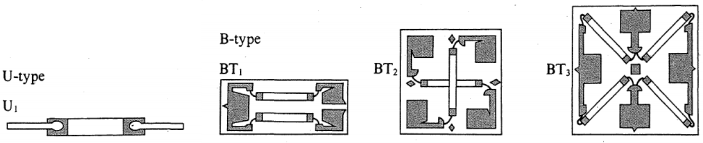
\includegraphics[width = 0.8\textwidth]{../img/diagram19.png}
  \caption{Some examples of semiconductor strain gauges}
\end{figure}
Characteristics of semiconductor strain gauges:
\begin{itemize}
  \item The material of the strain gauge reaches its elastic limit at about 4000 microstrain ($4000\times 10^{-6}$), much smaller than that of metals (typically 20000 microstrain)
  \item The gauge factor $G$ varies with high strain at high strain levels. i.e. the gauge is not linear
  \item The gauge factor varies with temperature
  \item The temperature coefficient of resistivity is large
\end{itemize}
\begin{figure}[H]
  \centering
  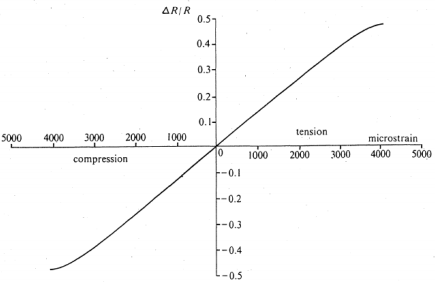
\includegraphics[width = 0.7\textwidth]{../img/diagram20.png}
  \caption{Change of resistance ratio with strain for a semiconductor strain gauge}
\end{figure}
\begin{figure}[H]
  \centering
  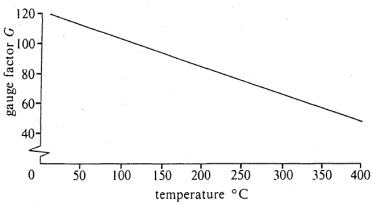
\includegraphics[width = 0.7\textwidth]{../img/diagram21.png}
\end{figure}
Negative effect of the temperature sensitivity of this type of strain gauge can be significantly reduced by using two gauges each consisting of two crystals connected in series. When two crystals are connected in series (but aligned in parallel), tensile of compressive strain applied to a gauge will produce an increase in the resistance of one crystal and a decrease in the other. Because the base material of each crystal is the same, their temperature coefficients of resistivity are approximately equal. In the configuration below, if the body experiences a tensile strain,
\begin{align}
  R_1 &= R(1+x)\\
  R_2 &= R(1-x)\\
  R_3 &= R(1-\nu x)\\
  R_4 &= R(1 + \nu x)
\end{align}
\begin{figure}[H]
  \centering
  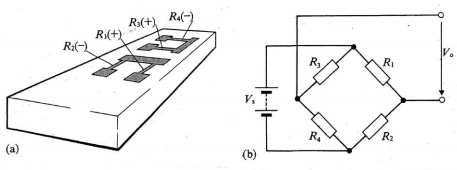
\includegraphics[width = 0.7\textwidth]{../img/diagram22.png}
\end{figure}
The bridge output voltage will thus be:
\begin{equation}
  V_0 = \frac{1}{2} V_S x (1 + \nu)
\end{equation}
Even if temperature increases, that affects all crystals equally. Also, changes in dimensions will cause $R_1 \uparrow$, $R_2 \downarrow$, $R_3 \uparrow$, $R_4 \downarrow$. Hence, no unbalance occurs. 
\section{Summary}
\begin{enumerate}
  \item Strain gauges utilise variability of resistance due to deformation
  \item Strain gauges are used in Wheatstone bridges with various gauge arrangements
  \item Bridge balance calculation is an essential part of the module
\end{enumerate}
\end{document}